\chapter{Different formulations of the same problem with examples}
\label{sec:ELBO}

AS MANY PICTURES AS POSSIBLE!!!

DO NOT FORGET COIN EXAMPLE

\section{Introduction}
\noindent For the remainder of this overview, we will always return to the specific example of determining the fairness of a coin, where the latent variable $z$ is the \textit{true} fairness of a coin, where $z=0.5$ indicates that the coin will show heads exactly half of the time. \\

\noindent $z$ - latent variables \\
\noindent $\theta$ - model parameters (i.e. latent variables. Therefore $\theta \in z$ (see below)) \\
\noindent $y$ - data, observation \\
\noindent $m$ - model (categorical variable) \\

\subsection{Notation}

\noindent Here I want to address a first point of confusion. Often we see different notations for the same thing, such as $q(z,\phi)$ and $q_{\phi}(z)$ for one and the same thing, and $p(y|m)$, or $p(y)$ for another thing. Sometimes we even see stuff like

\begin{equation}
p(x|\theta) = \frac{exp(-\frac{(x-\mu)^2}{2\sigma^2})}{\sqrt{2\pi \sigma^2}} = p(\theta|x),
\end{equation}

therefore

\begin{equation}
p(x|\theta) = p(\theta|x).
\end{equation}

\noindent What does all of this mean? Let's go through this step by step.

\subsubsection{\underline{$q(z,\phi)$ vs $q_{\phi}(z)$}}
In most of the literature, and throughout this treatment, $z$ is a latent (i.e. hidden) variable which is to be inferred, while $\theta$, $\phi$ often stands for the set of parameters of a model. In the case where our model is represented by a Gaussian distribution, these are be the mean and variance $\theta=\{\mu,\sigma\}$. So $\theta$ describes the parameters of the Gaussian distribution, while the distribution itself is a function of $z$ (EXPLANATORY PICTURE?). Therefore, the notation $p_\theta(z)$ might be useful as it tells us we are dealing with a distribution over $z$, parametrized by $\theta$, while notations such as $\Phi = \{ p_{\theta 1}, p_{\theta 2}, ... \}$ make clear we are dealing with a number of normal distributions, all with their own parameters. In inference problems, however, parameters themselves often have to be inferred themselves and can therefore be treated as latent variables. This is why we will always use notations like $p(z,\theta)$. At this point, we might as well include the latent variables $\theta$ into the set of other latent variables $z$.

\subsubsection{\underline{$p(y|m)$ vs $p(y)$}}

In the beginning this was very confusing to me, especially identities such as $p(x|theta) = p(\theta|x)$ as described before.  $p(\cdot |m)$ is to be understood as <<under a given model>>.


\emph{MEANING OF THE WORD <<MODEL>>}

\subsection{Energies and logarithms}

\noindent While we do not want to be bothered with the details for now, the main point to note that throughout the literature, the term \textit{energy} is used when talking about the logarithms of probability distributions $p(x)$. This comes from the fact that in statistical physics, the distribution of many interesting quantities of ensembles of particles (like the velocity distribution of air molecules in a box at a given temperature) can be described as $p(x) = \alpha \cdot e^{-E(x)}$, where $E(x)$ is the energy, given the quantity of interest $x$ (velocity, say). Beyond this rather simple analogy, there is not much more to it. The interested reader may refer to the \sref{sec:EnergiesAndLogs} for a more profound treatment of the physical origins of this.


\section{Variational Inference}

Given a specific model $m$, we have a probability distribution $p(x|m)$. For example, say $m = \mathcal{N}(\mu,\Sigma)$ (i.e. a normal distribution), then \\

\begin{align*}
p(x|m) = \frac{exp(-\frac{(x-\mu)^2}{2\sigma^2})}{\sqrt{2\pi \sigma^2}}.
\end{align*}

On its own, a probability distribution does not have any specific meaning when dealing with Bayesian inference, as in Bayesian inference a probability distribution can have many different meanings. When I talk about a \textit{model}, however, I generally think about the joint probability distribution $p(y,z)$ of observed data $y$ and hidden variables $z$, which consists of the \textit{likelihood} $p(y|z)$ and the \textit{prior} $p(z)$, which, in turn, are probability distributions of their own.

\noindent Given a specific model m, and parameters $\theta$ (e.g. $\theta = \{\mu, \sigma\}$), the \textit{model evidence} is 

$p(y|m) = \int p(y|\theta)p(\theta|m)d\theta$. 

\noindent The model evidence, or \textbf{marginal likelihood}, is the integral over all parameter values of the model. This can then be used to compare different models to select the best one, which is the one maximizing $p(y|m)$. [Murphy, page 158].  In the Free Energy formulation, the negative of the model evidence is interpreted as the \textbf{surprise}, which needs to be minimized (as the model evidence is to be maximized).\\

\noindent Once we did a number of different observations $y = \{y_1, y_2, ...\}$, we can compute the \textit{likelihood} $p(\theta|y,m)$ of a given model, which is a scalar value given a specific model and its parameters. The likelihood tells us (in arbitrary units), how \textit{likely} the parameters of our model are. For different parameters of the same model, and the same observations, we therefore get a function wrt to the parameters $\theta$, which is the \textit{likelihood function}:

\begin{equation}
p(\theta | y,m).
\end{equation}

This is a function of the model parameters $\theta$, and given a model and data we can choose those parameters which maximize that function which would then return the parameters which make observing the given data most likely (given the model). This is called \textit{Maximum Likelihood Estimation}. Now assume we want to perform Bayesian inference on the fairness of a coin. We are interested in the hidden variable $z$, which is equal to the actual fairness of the coin (probability of showing heads), and should be $0.5$ in the fairest case. After a number of coin flips $y={1,0,1,1...} (1=\text{heads})$, the Bayesian inference problem looks as follows: \\

\begin{equation}
p(z|y)= \frac{p(y|z)p(z)}{p(y)} \propto p(y|z)p(z),
\end{equation}

\noindent where we omit the $m$ for the model (for simplicity). We could write $p(y|z,m)p(z,m)$, but in a practical example this would just mean something like <<the likelihood and the prior, given that we know what form they are supposed to take>>. In a practical setting, the condition on $m$ is met just by knowing what forms those distributions are to take, which you need to know in order to be able to actually compute something with them, obviously. Confusingly enough, $p(y|z)$ is also called the likelihood and must not be confused with the likelihood function above. While the nominator is basically our <<view of the world>> (i.e.) our model, and is strongly dependent on our beliefs, the denominator $p(y)$ gives the <<true>> probability of the observed data (or \textit{evidence}) and is generally not accessible to us. However this shall not further concern us, as it is just a normalizing constant and does not influence the inference process, as most inference processes boil down to finding maxima of functions and are quite independent of their actual value. $p(z)$ is the \textit{prior} over our hidden variable $z$ and constitutes our prior believe of what value $z$ is likely to take on. In the unbiased case, we might choose $p(z)$ to be a Beta distribution around $0.5$. The \textit{likelihood} $p(y|z)$ is the Bernoulli distribution (for one observed coin flip) or, equivalently, the binomial distribution for a number n of coin flips. Our goal is to find out $p(z|y)$ (Bishop page 463). But this is not always easily doable (WHY). Therefore, we define an \textit{approximate posterior} $q(z)$, which we will try to bring as close to $p(z|y)$ as possible. We want thus to minimize $D_{KL}(q(z)||p(z|y))$. This is still pretty complicated, as evaluating $p(z|y)=\frac{p(y|z)p(z)}{p(y)}$ would require the (unknown) normalization constant $p(y)$. Therefore we try to minimize the following instead\footnote{$D_{KL}(f(x)||g(x))$ is the \textit{Kullback-Leibler} divergence. It is a similarity measure between probability distributions and is defined as $D_{KL}(f(x)||g(x))= \int f(x)\log\frac{f(x)}{g(x)} dx$. It is probably a good idea to remember this definition by heart. Note how it cannot generally be used as a similarity measure between \textit{functions}, as $\log\frac{f(x)}{g(x)}$ will then not be guaranteed to be positive.}:

\begin{equation}
D_{KL}(q(z)||p(z,y)) = \int q(z)\log \frac{q(z)}{p(z,y)} = F[q(z)]
\label{eq:FE}
\end{equation}[Murphy, page 734], which is the \textit{variational free energy}. We take a second to let that sink in: \textbf{The Variational Free Energy is the distance between the approximate posterior and the (auxiliary) joint distribution}\footnote{The term \textit{Free Energy} comes first and foremost from the fact that it looks very similar to the concept of Free Energy in statistical physics. For a short introduction to the concept of Free Energy in statistical physics, see \sref{sec:FE_app}.}. Reordering that equation:

\begin{equation}
\int q(z)\log \frac{q(z)}{p(z,y)} dz= \int q(z)\left[ \log \frac{q(z)}{p(z|y)} - \log p(y) \right]dz,
\end{equation}

\noindent and thus\footnote{Using $\int dz q(z)\log p(y) = p(y)$, as $q(z)$ is a probability distribution.}

\begin{equation}
D_{KL}(q(z)||p(z,y)) = D_{KL}(q(z)||p(z|y)) - \ln p(y).
\end{equation}

\noindent Therefore, \textbf{minimizing the variational free energy by tweaking $q(z)$ minimizes the distance between the approximate posterior and the true posterior}. This is true, as changing $q(z)$ does not have an effect on $\ln p(y)$ and can therefore be considered a constant in this context. \\

\noindent As $D_{KL}$ is always greater than zero, the negative of the Free Energy is a lower bound of the model evidence $p(y)$ (sometimes $p(y|m)$). This lower bound is sometimes called the \textit{evidence lower bound}, or \textit{ELBO}.

\noindent Rewriting \eref{eq:FE}, we find the following:

\begin{equation}
 F[q(z)] = - \left<\ln p(y,z) -\ln q(z) \right>_{q(z)},
\end{equation}

\noindent which reformulates the free energy in terms of an energy term and an entropy term. FEW WORDS ON ENTROPY TERM

\section{ToDo}

1) The unrestricted Free Energy Principle is Bayesian Inference [Samuel Gershman: What does the free energy principle tell us about the brain?]

2) Bayesian Central Limit Theorem: justification for Gaussian assumption [Gershman]

3) Laplace approx: Linearize Free Energy around the posterior mode, as Free Energy is usually not tractable [Gershman]

4) Predictive Coding as an aspect of FEP [Gershman]

5) Active Inference: Minimization of expected Free Energy

\chapter{Hamilton's Principle}

As stated in the previous chapters, during Bayesian Inference, we want to find the true posterior distribution $p(z|y)$. For reasons of simplicity, we assume that all probability distributions are Gaussian distributions. This is called the \textit{Laplace approximation}. In this case, all we are really interested in is the mean of the distribution $p(z|y)$, ignoring the variance for a moment. The mean $\mu$ of $p(z|y)$ is the coordinate where the distribution assumes its maximum. Numerically, this maximum can be reached via a gradient ascent scheme:

\begin{align*}
\dot{\mu_g} = \frac{d}{dz} \ln p(z|y),
\end{align*}
where the subscript $g$ stands for <<guessed>>, as the true mean is always at the true mode of the energy $\ln p$, while we are trying to approach that true mean via gradient ascent of our guessed mean $\mu_g$. Importantly,  $\dot{\mu_g}$ does not stand for the <<natural>> evolution of $\mu_g$ with time, but for the change we need to apply to it in order to make it closer to the mode of the energy. \\

\noindent The above case is true for static systems, but what if $p(z|y)$ changes over time? Answer:

\begin{align*}
\dot{\mu_g} = D\mu_g + \frac{d}{dz} \ln p(z|y),
\end{align*}

where now $D\mu$ is the <<natural>> time-evolution of the mean. This corrects the guessed mean such that it accounts for the distance to the actual mean as well as for their natural time-evolution.
\begin{center}
\begin{figure}
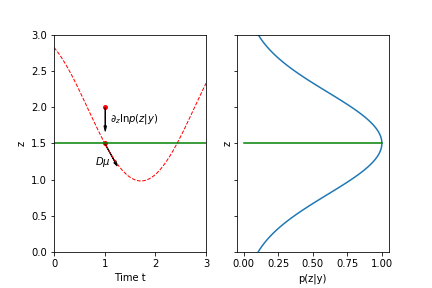
\includegraphics[scale=0.7]{images/FE_ex_4}
\caption{The true mode of the probability distribution $p(z|y)$ is at $z=1.5$ (green line), while the <<guessed>> mean is at $z=2$. The dashed red line describes the time evolution of the mode of the probability distribution, which is described by the differential operator $D$ acting on $\mu$. The correction $\dot{mu}$ to be applied to the guessed mean is then $\frac{d}{dz} \ln p(z|y) + D\mu$.}
\end{figure}
\end{center}
[Friston \& Kiebel, Predictive Coding under the free energy principle; Friston: Hierarchical models in the brain].